\chapter{Results}
What are the measurement/model results

\section{Acoustic measurements}

Figure \cref{fig:period_1k} shows a periodogram of the recorded audio signal with a 1kHz input on X2. This periodogram is a fourier transform of the recorded audio 
\begin{figure}
    \centering
    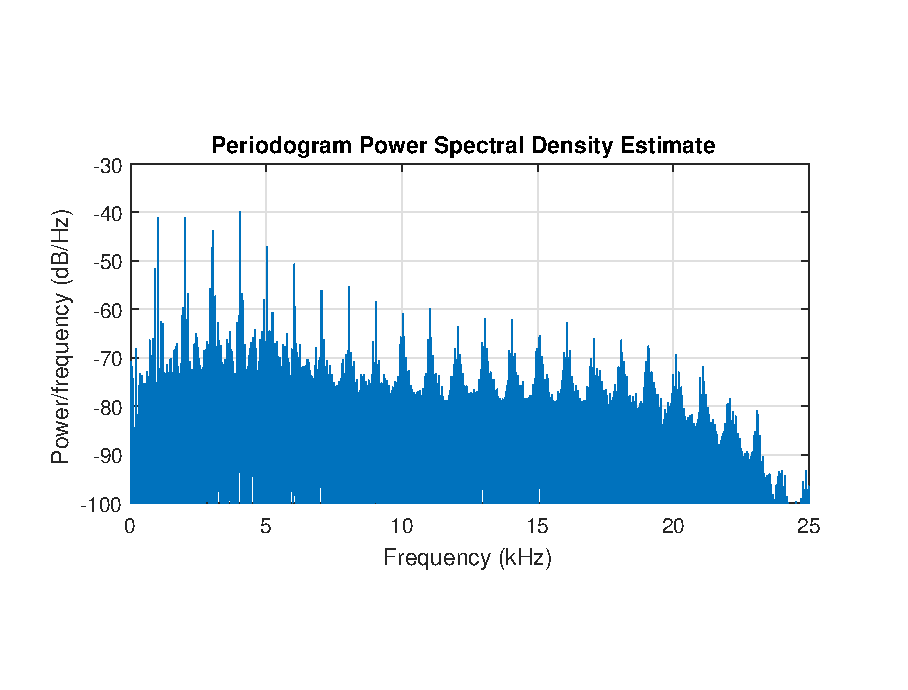
\includegraphics[trim={0cm 1.6cm 0cm 2cm},clip,width=\textwidth]{img/Periodogram_1khz-09.eps}
    \caption{Periodogram of 1kHz recorded tone}
    \label{fig:period_1k}
\end{figure}

\begin{figure}
    \centering
    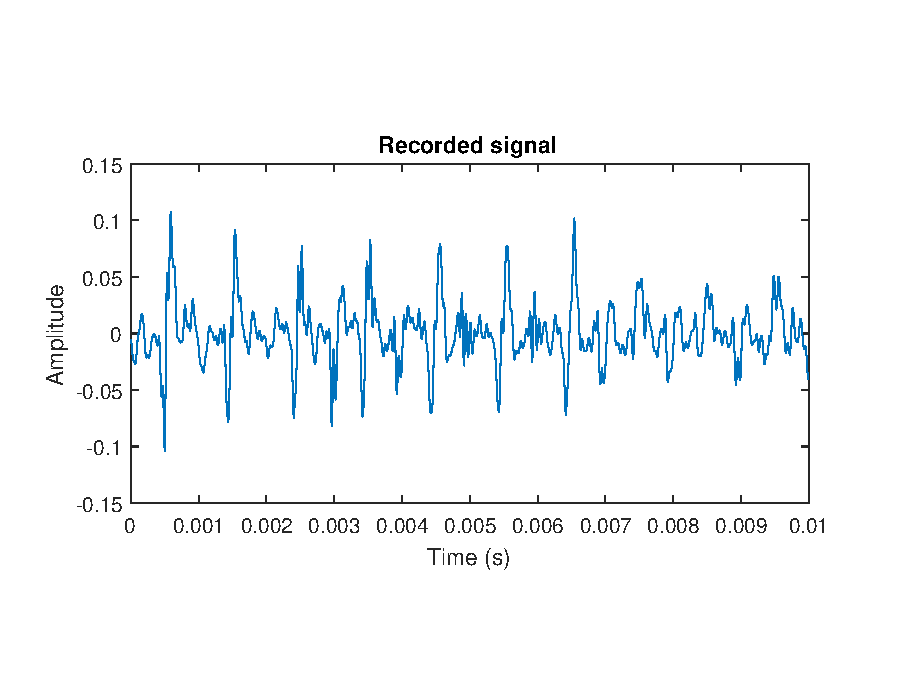
\includegraphics[trim={0cm 1.6cm 0cm 2cm},clip,width=\textwidth]{img/Recorded_1khz-09.eps}
    \caption{Time domain plot of 1kHz recorded tone}
    \label{fig:recorded_1k}
\end{figure}

%\begin{table}[]
%    \centering
%    \begin{tabular}{c|c|c|c|c|c|c|c|c|c|c|c|c|c|c|c|c|c|c|c|c|c|c}
%        Frequency (Hz)      & 1k  & 2k  & 3k  & 4k  & 5k  & 6k  & 7k  & 8k  & 9k  & 10k & 11k & 12k & 13k & 14k & 15k & 16k & 17k & 18k & 19k & 20k & 21k & 22k \\
%        Amplitude (dB/Hz)   & -41 & -41 & -44 & -40 & -47 & -51 & -55 & -55 & -58 & -60 & -60 & -64 & -62 & -62 & -65 & -62 & -66 & -66 & -67 & -70 & -72 & -80 \\
%    \end{tabular}
%    \caption{Caption}
%    \label{tab:my_label}
%\end{table}

\begin{table}[]
    \centering
    \begin{tabular}{c|c}
        Frequency (Hz) & Amplitude (dB/Hz) \\
        1k  & -41 \\
        2k  & -41 \\
        3k  & -44 \\
        4k  & -40 \\
        5k  & -47 \\
        6k  & -51 \\
        7k  & -55 \\
        8k  & -55 \\
        9k  & -58 \\
        10k & -60 \\
        11k & -60 \\
        12k & -64 \\
        13k & -62 \\
        14k & -62 \\
        15k & -65 \\
        16k & -62 \\
        17k & -66 \\
        18k & -66 \\
        19k & -67 \\
        20k & -70 \\
        21k & -72 \\
        22k & -80
    \end{tabular}
    \caption{Amplitudes of the harmonics}
    \label{tab:1k_amps}
\end{table}

\Cref{fig:tones} shows the recorded signal compared to a signal generated with the amplitudes read from the periodogram of the recorded signal and shown in \cref{tab:1k_amps}.

\begin{figure}
    \centering
    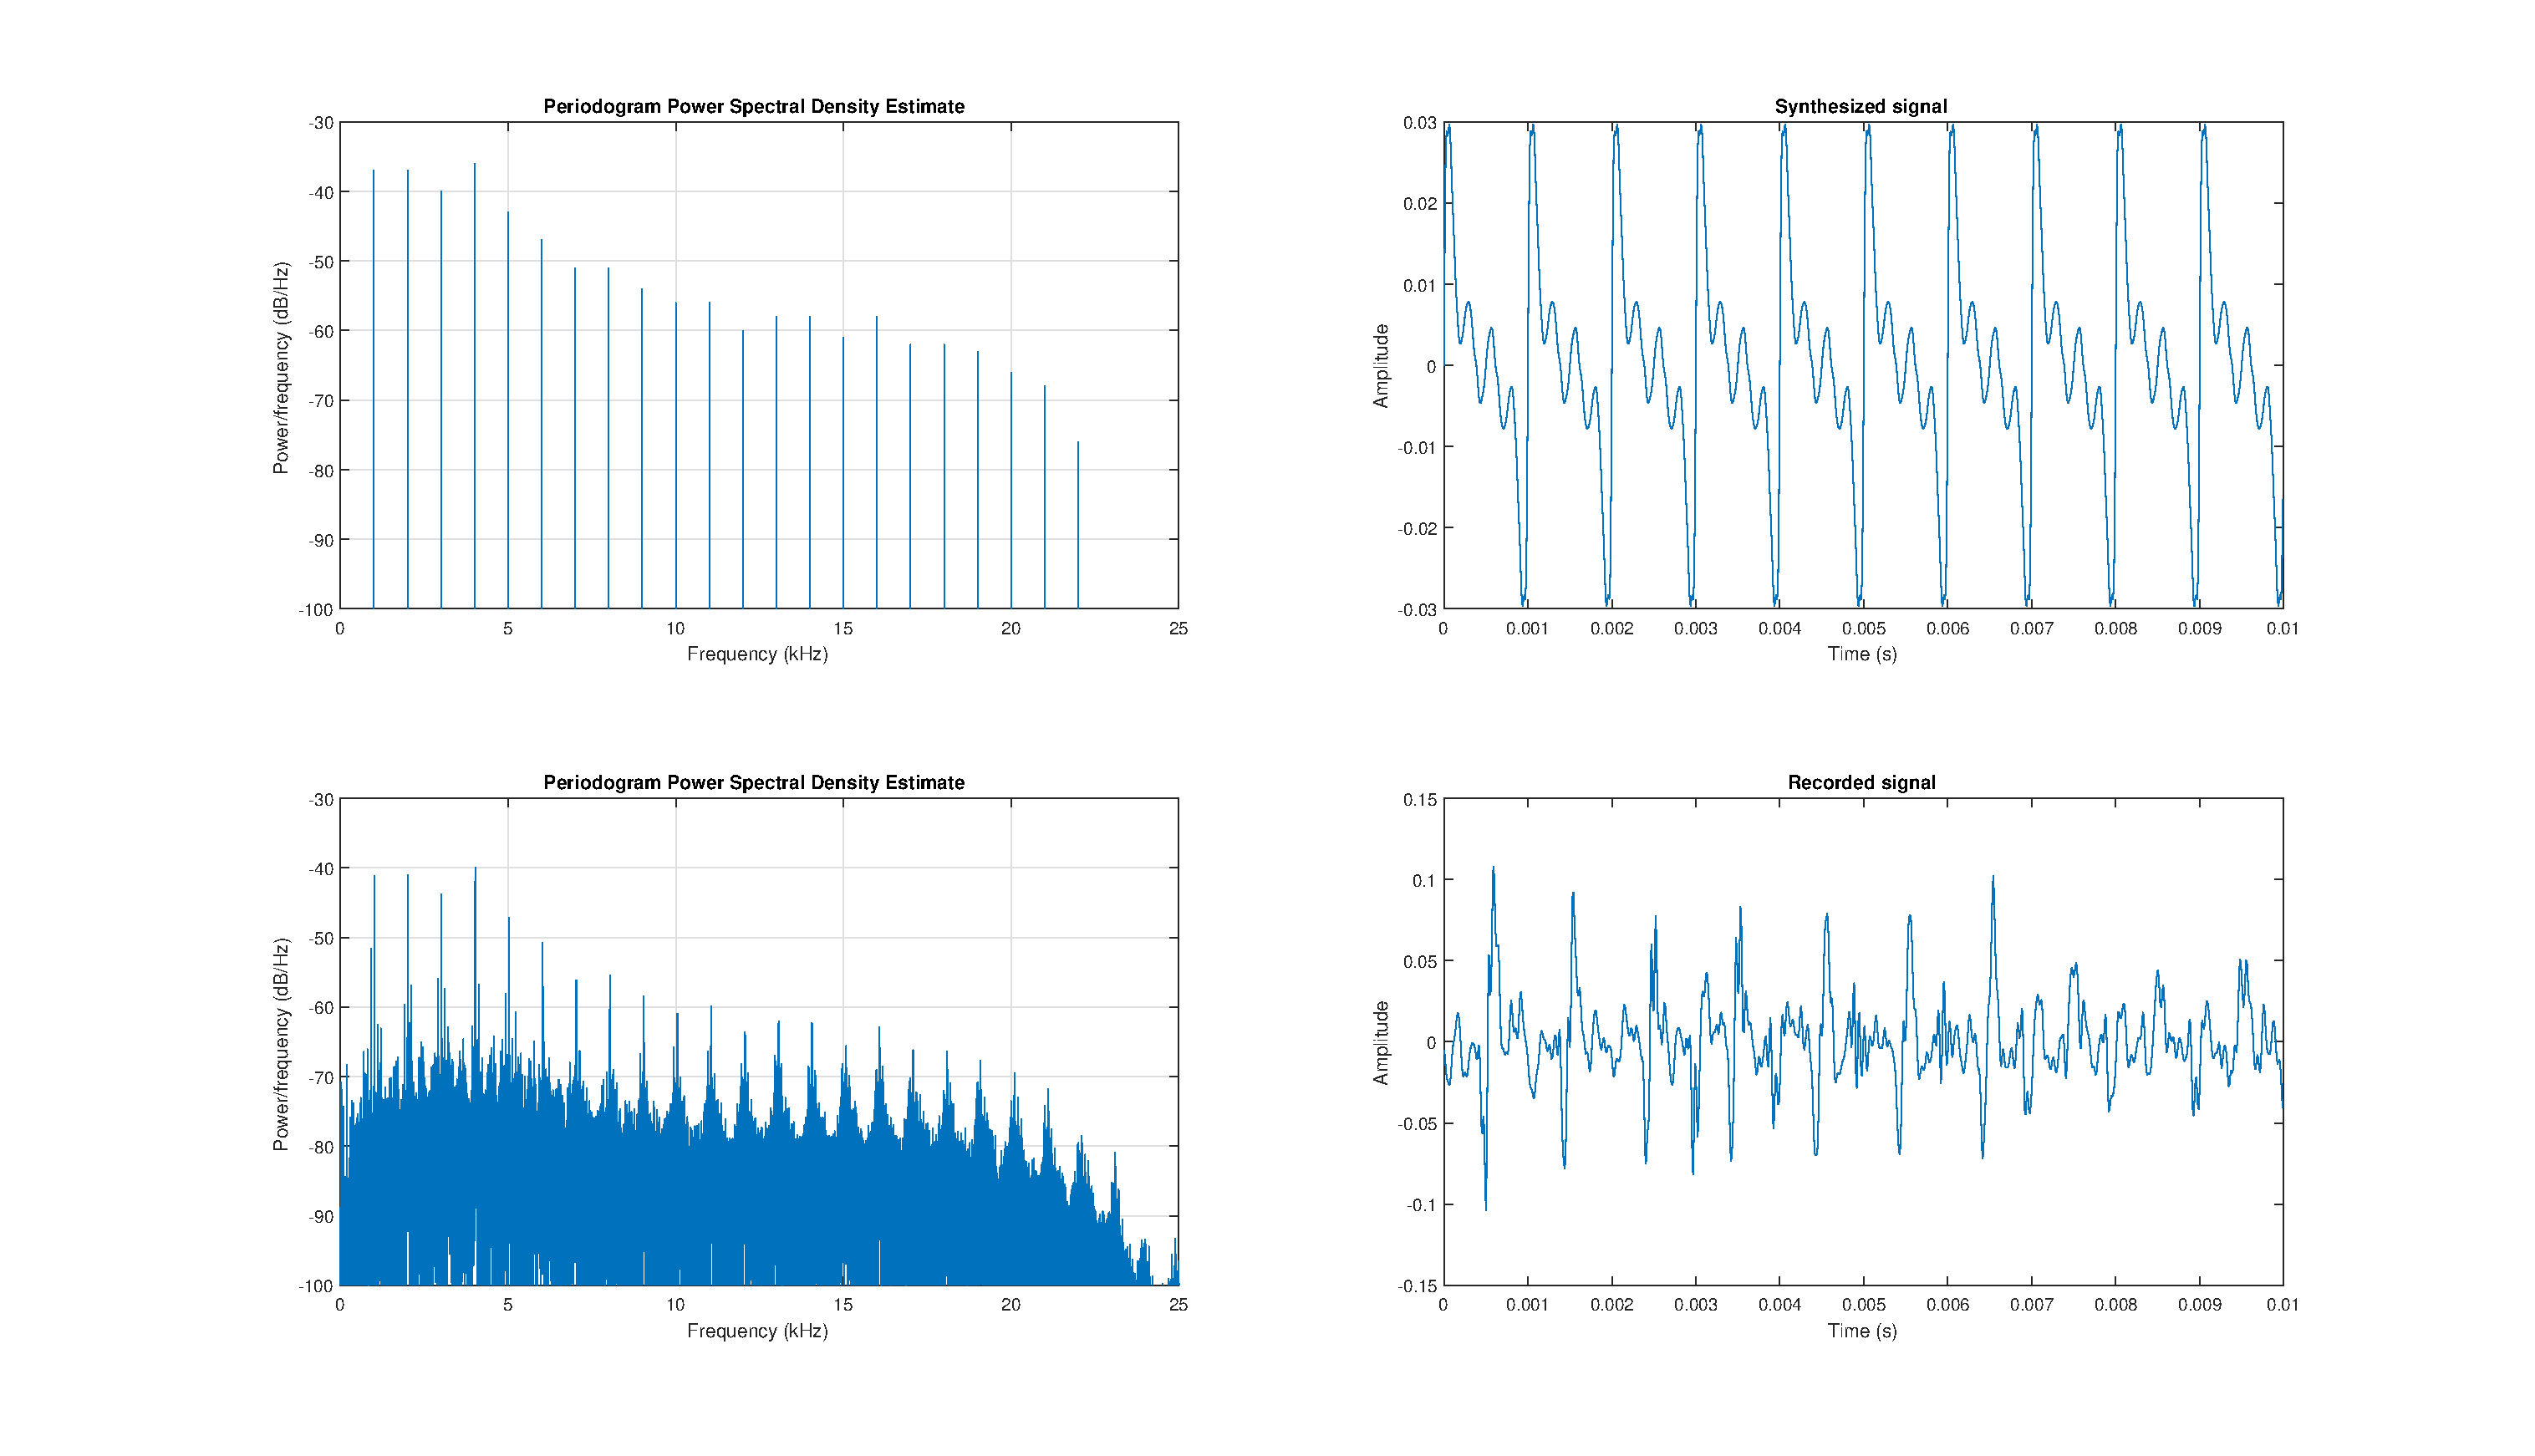
\includegraphics[trim={0cm 1.6cm 0cm 2cm},clip,width=\textwidth]{img/tones.eps}
    \caption{Comparison of recorded tone and synthesized tone}
    \label{fig:tones}
\end{figure}

From this figure we see that the reconstructed signal matches well with the exception of the noise.